%Experimental Results and Analysis – in this section, you should show the quantitative results – charts and tables. Analyze the results by explaining and highlighting what is important on them in terms of your goals and what is bad. You should explain the strange results too.

%V ďalšej časti prezentujte vlastný prínos a vlastné výsledky porovnajte s výsledkami iných. Charakterizujte použité metódy.
%Vyhýbajte sa používaniu žargónu.
%Používajte starú múdrosť: 1 obrázok je viac než 1000 slov.

\subsection{Handwritten Digits} 
\label{sec:results-digits} 

(\ref{sec:datasets-digits}) 

%===============================================================
%===============================================================
%===============================================================
\subsubsection{Two learning rates} 
\label{sec:tlr-digits} 

%Purpose: 
%======== (3D) L1 x L2 x patSuccF =========
%======== (3D) L1 x L2 x epochs =========
\begin{figure}[H]
  \centering
  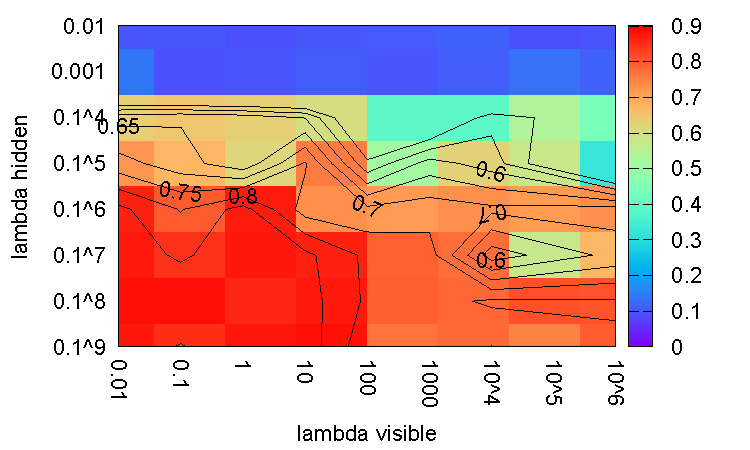
\includegraphics[width=0.60\textwidth]{img/tlr-digits-psf.pdf} 
%  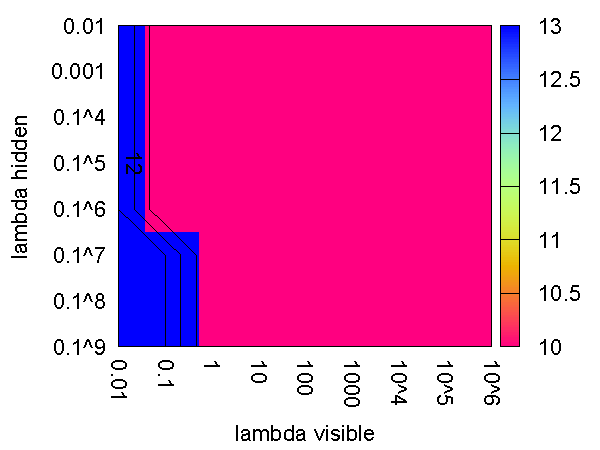
\includegraphics[width=0.49\textwidth]{img/tlr-digits-epoch.pdf}     
  \caption{TLR performance on the \emph{digits} task for $\mu = 0.01$.}
  \label{fig:results-tlr-digits-success}
\end{figure}

%======== (2D) best TLR on ALL_SUCC x epoch (std-dev) ==========
\begin{figure}[H]
  \centering
  
\includegraphics[width=0.45\textwidth]{img/placeholder.png}  %TODO    
  \caption{TLR success evolution for the \emph{digits} task.}
  \label{fig:results-tlr-digits-epoch} 
\end{figure}

%===============================================================
%===============================================================
%===============================================================
\subsubsection{Comparison} 
\label{sec:results-cmp-digits} 
TODO simulation + plots~(\ref{sec:datasets-digits}) 

For TLR, BAL, GeneRec + known performers 
TODO: table: best parameter setting networks with hidden.size= constant (success, epoch, stddev) / model \\

\begin{table}[H] 
  \centering
    \begin{tabular}{|l|l|l|l|l|}
    \hline
    Algorithm (section)&$\lambda_h$&$\lambda_v$&$patSucc^F$ &Epochs\\ %&SEM(success) \\
    \hline
    BAL TLR~(\ref{sec:our-tlr})& & & & \\ %&1.52e+08\\
    \hline 
    \end{tabular}
  \caption{Comparing performance of different models on the \emph{digits} task with 300 hidden neurons.} 
  \label{tab:results-cmp-digits}
\end{table}

\paragraph{Backward representations.} 
(\ref{sec:our-backward-repre}) 

TODO 3x 10x backward digit representations 

\begin{figure}[H]
  \centering
  
\includegraphics{../presentation/img/dig_0.png} %TODO 
  
\includegraphics{../presentation/img/dig_1.png} 
  
\includegraphics{../presentation/img/dig_2.png} 
  
\includegraphics{../presentation/img/dig_3.png} 
  
\includegraphics{../presentation/img/dig_4.png} 
  
\includegraphics{../presentation/img/dig_5.png} 
  
\includegraphics{../presentation/img/dig_6.png} 
  
\includegraphics{../presentation/img/dig_7.png} 
  
\includegraphics{../presentation/img/dig_8.png} 
  
\includegraphics{../presentation/img/dig_9.png} 
  \caption{Backward representations on \emph{digits} for GeneRec.}
  \label{fig:results-backward-repre-generec}
\end{figure}


%===============================================================
%===============================================================
%===============================================================
\subsubsection{Backward representations} 

\label{sec:our-backward-repre}

The method of \emph{backward representations} for \emph{hetero--associative} tasks, i.e.~tasks which have multiple inputs for the same output, is to \emph{depict} the backward activation of all possible outputs. In case of BAL~(\ref{sec:models-bal}) the backward representations are all possible values of $x^{\rm B}$. For example the backward representation of digit "8" in TLR~(\ref{sec:our-tlr}) is show on figure~\ref{fig:our-backward-repre}. 

\begin{figure}[H]
  \centering
  
\includegraphics[width=0.2\textwidth]{img/tlr-digit-8.png} %TODO 
  \caption{Backward representation of digit "8" in TLR.}
  \label{fig:our-backward-repre}
\end{figure}

%======== (2D) for best network vs. sample digits
\begin{figure}[H]
%TODO rotate 
  \centering
  
\includegraphics[width=0.45\textwidth]{img/tlr-digits.png}    
  \caption{Best TLR backward representations for the \emph{digits} task.}
  \label{fig:results-tlr-digits-backward} 
\end{figure}
